\documentclass{article}


% if you need to pass options to natbib, use, e.g.:
%     \PassOptionsToPackage{numbers, compress}{natbib}
% before loading neurips_2023

% ready for submission
\usepackage[final]{neurips_2023}

% to avoid loading the natbib package, add option nonatbib:
%    \usepackage[nonatbib]{neurips_2023}


\usepackage[utf8]{inputenc} % allow utf-8 input
\usepackage[T1]{fontenc}    % use 8-bit T1 fonts
\usepackage{hyperref}       % hyperlinks
\usepackage{url}            % simple URL typesetting
\usepackage{booktabs}       % professional-quality tables
\usepackage{amsfonts}       % blackboard math symbols
\usepackage{nicefrac}       % compact symbols for 1/2, etc.
\usepackage{microtype}      % microtypography
\usepackage{xcolor}         % colors
\usepackage{graphicx}       % graphics

\renewcommand{\thesection}{\arabic{section}.)}
\renewcommand{\thesubsection}{\alph{subsection}.)}



\begin{document}



\section{Audio Features}
\label{sec:Audio Features}


\subsection{Which audio features appear useful? Select only the most relevant ones or perform a down projection for the next steps.}
\label{sec:Audio Features:a}

As a method to extract the most important audio features, PCA was chosen.

The first step was to flatten them into a single array to make them usable for PCA. Using flattened data, the goal was to reach a cumulative explained variance of 95\%.

\begin{figure}[htbp]
    \centering
    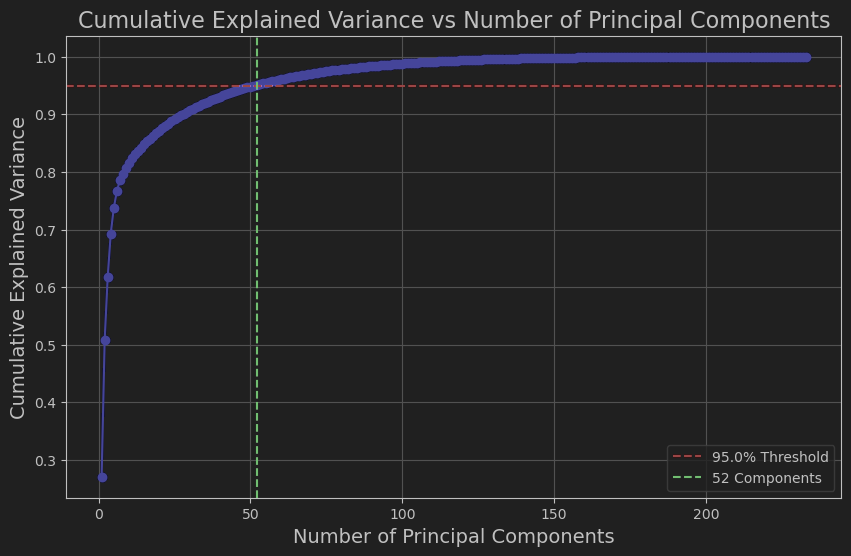
\includegraphics[width=0.5\linewidth]{Cumulative Explained Variance.png}
    \caption{Cumulative Explained Variance using PCA on the audio features}
    \label{fig:Cumulative Explained Variance}
\end{figure}

The threshold is reached with 52 Principle Components. Now the 10 most important feature groups (embeddings, ZCR, mel-spectrogram, mfcc, etc.) of each component are counted. 

\textbf{Top contributing feature groups across the first 52 components:}

Feature Group: mfcc, Count: 338;
Feature Group: melspectrogram, Count: 82;
Feature Group: embeddings, Count: 76;
Feature Group: contrast, Count: 14;
Feature Group: centroid, Count: 3;
Feature Group: energy, Count: 2;
Feature Group: power, Count: 1;
Feature Group: flatness, Count: 1;
Feature Group: bandwidth, Count: 1;
Feature Group: zerocrossingrate, Count: 1;
Feature Group: flux, Count: 1

As a result, $\Delta$-mfcc and $\Delta\Delta$-mfcc can be ignored.

\subsection{Extract a fixed-length feature vector for each annotated region as well as for all the silent parts in
between. }
\label{sec:Audio Features:b}.

First the unimportant features are excluded and the annotated, as well as unannotated parts get extracted.
The snippets of the audio features are concatenated into a single array, where the first [:len(X)] elements are annotated and the rest unannotated features. T-SNE is then used to create a 2-dimensional vector for each section.

\begin{figure}[htbp]
    \centering
    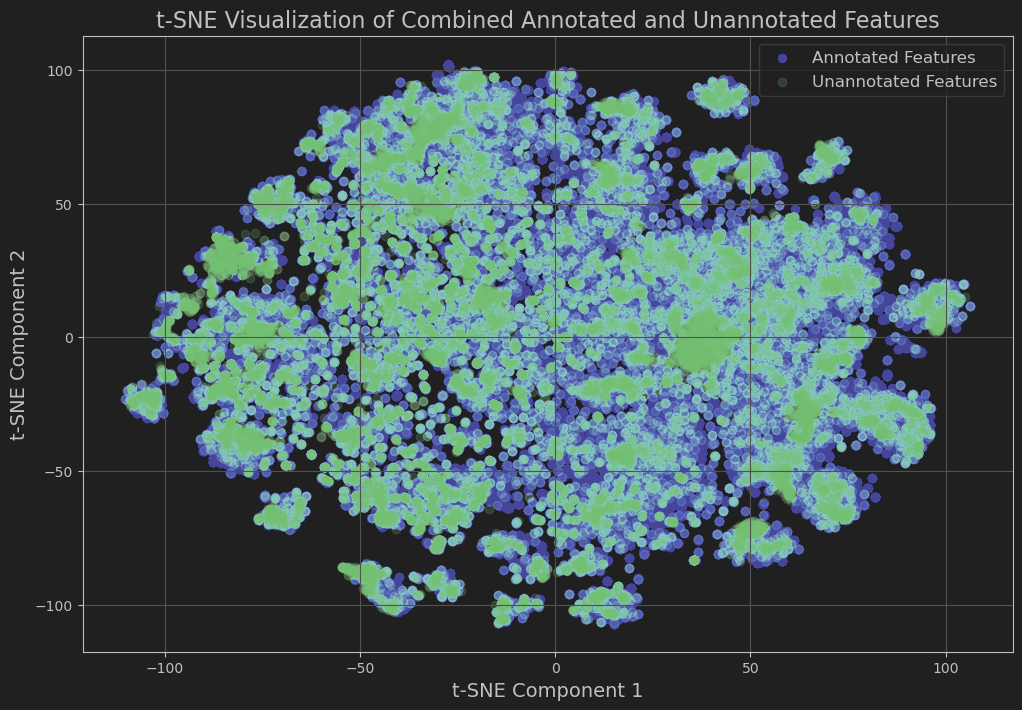
\includegraphics[width=0.5\linewidth]{Audio Features T-SNE.png}
    \caption{Audio Features T-SNE}
    \label{fig:Audio Features T-SNE}
\end{figure}

\subsection{Cluster the audio features for the extracted regions. Can you identify meaningful clusters of audio
features? Do the feature vectors of the silent regions predominantly fall into one large cluster?}
\label{sec:Audio Features:c}

K-means was used to cluster the audio features. The clustering was applied on the raw data instead of the t-SNE down projection since it yielded a better differentiation of annotated and unannotated features.

\begin{figure}[htbp]
    \centering
    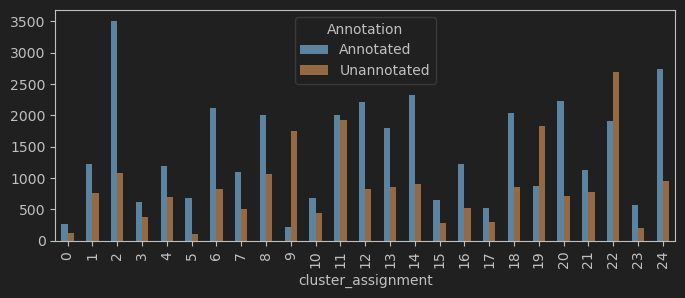
\includegraphics[width=0.5\linewidth]{Clustered Audio Features.png}
    \caption{Clustered Audio Features}
    \label{fig:Clustered Audio Features}
\end{figure}
While cluster 9 consists almost only of unannotated features, it is not so clear for all the other clusters. This is probably due to the fact, that most unannotated parts are either not completely silent or are small gaps between annotations that should still be part of the annotation.

\end{document}